\documentclass[12pt]{article}

\usepackage[margin=1in]{geometry}
\usepackage{amsfonts,amsmath,amssymb}
\usepackage{multicol}

\usepackage{graphicx}
\usepackage{float}
\usepackage[nottoc, notlot, notlof]{tocbibind}
\usepackage{hyperref}
\usepackage{enumitem}
\usepackage{caption}
\usepackage{subcaption}
\usepackage[T1]{fontenc}
\usepackage[utf8]{inputenc}
\usepackage{xcolor}
\newcommand{\leavealine}
{\vskip 0.5cm}


% for equation box
\usepackage{color}
\definecolor{myblue}{rgb}{.8, .8, 1}

\usepackage[most]{tcolorbox}
\tcbset{
	enhanced,
	colback=myblue!100!white,
	boxrule=0.1pt,
	colframe=myblue!100!black,
	fonttitle=\bfseries
}
%until here

% for python code
\usepackage[utf8]{inputenc}

% Default fixed font does not support bold face
\DeclareFixedFont{\ttb}{T1}{txtt}{bx}{n}{12} % for bold
\DeclareFixedFont{\ttm}{T1}{txtt}{m}{n}{12}  % for normal

% Custom colors
\definecolor{deepblue}{rgb}{0,0,0.5}
\definecolor{deepred}{rgb}{0.6,0,0}
\definecolor{deepgreen}{rgb}{0,0.5,0}

% \usepackage{listings}

% Python style for highlighting
\usepackage[utf8]{inputenc}

% Default fixed font does not support bold face
\DeclareFixedFont{\ttb}{T1}{txtt}{bx}{n}{12} % for bold
\DeclareFixedFont{\ttm}{T1}{txtt}{m}{n}{12}  % for normal

\DeclareSymbolFont{matha}{OML}{txmi}{m}{it}% txfonts
\DeclareMathSymbol{\varv}{\mathord}{matha}{118}
% Custom colors
\usepackage{color}
\definecolor{deepblue}{rgb}{0,0,0.5}
\definecolor{deepred}{rgb}{0.6,0,0}
\definecolor{deepgreen}{rgb}{0,0.5,0}
\definecolor{almostwhite}{rgb}{0.99,0.99, 0.99}

\usepackage{listings}

% Python style for highlighting
\lstset{
	basicstyle  =   \footnotesize,
	keywordstyle    = \color{deepred}\bfseries,
	stringstyle     = \color{strings},
	identifierstyle = \color{black},
	commentstyle    = \color{deepgreen},
	breaklines=true,
	numbersep=-10pt,
	stepnumber=1,
	showspaces=false,
	escapechar=§,
	showstringspaces=false,
	showtabs=false,
	frame=single,  
	rulecolor=\color{black},
	tabsize=4,              
	captionpos=t,           
	breaklines=true,
	breakatwhitespace=false,
	numbers=left,
	extendedchars=\true,
	emph=[3]{href, Particle, Boris_update, Field, uniform_E_field, radial_E_field, uniform_B_field, helmholtz_coil_B_field, two_helmholtz_B_field, Sampler, sample_uniform_position, sample_uniform_velocity, sample_velocity_uniformKE, sample_Maxwellian_velocity, sample_parabolic_velocity},
	emphstyle=[3]{\color{deepblue}},
	backgroundcolor=\color{almostwhite},
	language=Python 
}

%until here

\begin{document}
	
	\fontfamily{ppl}\selectfont 
		\begin{center}
			\large{\textbf{MEE4099 Capstone Project}} \hspace{1cm}\large{\textbf{Review 1 Report}} \\
			 \large{Project Title:} \\ \Large{\textbf{Magnetic Mirror Effect in Magnetron Plasma:}} \\
			\Large{\textbf{Modeling of Plasma Parameters}} \\
		\end{center}
		%\color{blue}
	\textbf{Project ID:} 21BTECH10051 \\
	\textbf{Team Members:} \\
	18BEM0145 Sashi Kant Shah \\
	18BME2104 Kaushal Timilsina \\
	18BME2109 Hrishav Mishra \\
	
	\noindent \textbf{Internal Guide:} \\
	Professor Sitaram Dash
	
	\section{Introduction}
	One of the team members- 18BME2104 Kaushal studied the class MEE4005 Surface Engineering taught by Professor Sitaram Dash- our internal guide during the Fall Semester 2021. Many interesting plasma based surface engineering techniques were studied during the class, one such technique being Magnetron Sputtering. This inspired the study of plasma in this project.
	
	\subsection{Plasma}
	One comes across many definitions of plasma including: Fourth state of matter, Ionized gas, etc. However, it is best to describe plasma with some characteristic parameters, when one attempts to describe a plasma quantitatively. Some quantities that help define a plasma are:
	\begin{enumerate}
		\item Number density, $n$ \\
		Number density of a plasma describes the number of particles per unit volume. Plasma contains charged particles or ionized species. However, a plasma might at the same time also contain neutral atoms and molecules but also particles of different species- charged and neutral. If multiple species are contained in a plasma system, number densities of each species could be used to describe the system. For example, a plasma may contain electrons, charged ions and neutral atoms and molecules. Mass density $\varrho$ is defined as $\varrho := m n$ and is often used alongside number density, where $m$ is the mass of the species.
		
		\item Ionization, $\alpha$ \\
		Defined as $\alpha := \frac{\displaystyle n_{charged}}{\displaystyle n_{charged} + n_{neutral}}$, the ionization of a plasma describes the fraction of charged particles, with $\alpha = 1$ meaning that all the particles are charged and $\alpha = 0$ meaning that all the particles are neutral.
		
		\item Temperature, $T$ \\
		The temperature of a plasma describes the average kinetic energy of the particles in the plasma. When a gas is ionized to form a plasma, the ionization $\alpha$ can depend on the temperature of the plasma.
		
		\item Mean free path, $\lambda_{mfp}$ \\
		The gas-like behavior of a plasma is characterized by mean free path of particles much larger than the scale of the plasma. The mean free path is influenced by the temperature of the plasma. The mean free path and the thermal velocity of the particles as described by the temperature, are related by the timescale of collisions as $\lambda := v_{th} \tau$ where $\tau$ is the timescale of collisions. 
		
		\item Debye Length, $\lambda_{D}$ \\
		In a plasma, electrostatic Coulomb interactions between charged particles compete with random thermal speed of the particles described by the temperature of the plasma. The Debye sphere is an imaginary sphere around a charged particle, where oppositely charged particles are attracted and in doing so screen the charge of the central particle to the outer plasma so that the electrostatic influence of a particle is limited to the Debye sphere surrounding it. This is why plasma's are often said to be Quasi-neutral as charge screening leads to a neutral behavior electrostatically on a scale much larger than the Debye length. The Debye length is defined as the radius of the Debye sphere.
		
		\item Plasma beta parameter, $\beta$ \\
		The beta parameter defined as $\beta := \frac{\displaystyle 8 \pi n T}{\displaystyle B^{2}}$ describes the ratio of the thermal and magnetic energies of the plasma, as particles in random thermal motions compete with the Lorentz force.
		
	\end{enumerate} 
		Many other parameters describe a plasma including several electrodynamic quantities.
	
	\subsection{Laboratory Plasma}
	Laboratory plasmas are often characterized by some properties like:
	\begin{itemize}[itemsep=0cm]
		\item High ionization fraction
		\item Sub atmospheric pressure required to sustain ionization
		\item Temperature range : 1000 - 30000 K
	\end{itemize}

	\noindent Many surface engineering processes use plasmas to obtain high performance coatings. Some processes that use plasma are:
	\begin{enumerate}[itemsep=0cm]
		\item Plasma Immersion Ion Implantation
		\item Plasma Enhanced Chemical Vapor Deposition
		\item Magnetron Sputtering (PVD)
		\item Air Plasma Spray (Spray technique)
		\item Plasma Transferred Arc (Hardfacing technique)
	\end{enumerate}
	
	\subsection{Physical Vapor Deposition}
	Physical Vapor Deposition(PVD) is a family of surface engineering techniques where thin film coatings are grown on the surface of a specimen, in a vacuum chamber. Particles from a vapor move around on the surface of the specimen as random walkers and eventually get trapped in strained pockets producing nucleation site for the growth of a film. Most PVD techniques fall under either of the two catgories:
	\begin{enumerate}
		\item Evaporation techniques \\
		Evaporation techniques involve heating the material to  to a high temperature when it forms vapor and the particles in the vapor are coated on the substrate. It is for that reason that evaporation techniques are called hot techniques. Semiconductors like Si/Ge, insulators like oxides and metals like Tungsten are often coated on substrates using evaporation techniques. 
		
		\item Sputtering techniques \\
		Sputtering techniques on the other hand are known as cold techniques. Sputtering techniques use a high energy beam to remove material from a target and the removed material is coated on the required substrate.
		
	\end{enumerate}

	\subsection{Magnetron Sputtering}
	Magnetron sputtering is a sputtering technique where the sputtered ions form a magnetically confined plasma. The plasma, controlled by magnetic fields, transports the ions to the surface of the substrate forming the coating. 
	
	
	\begin{figure}[H]
		\begin{center}
			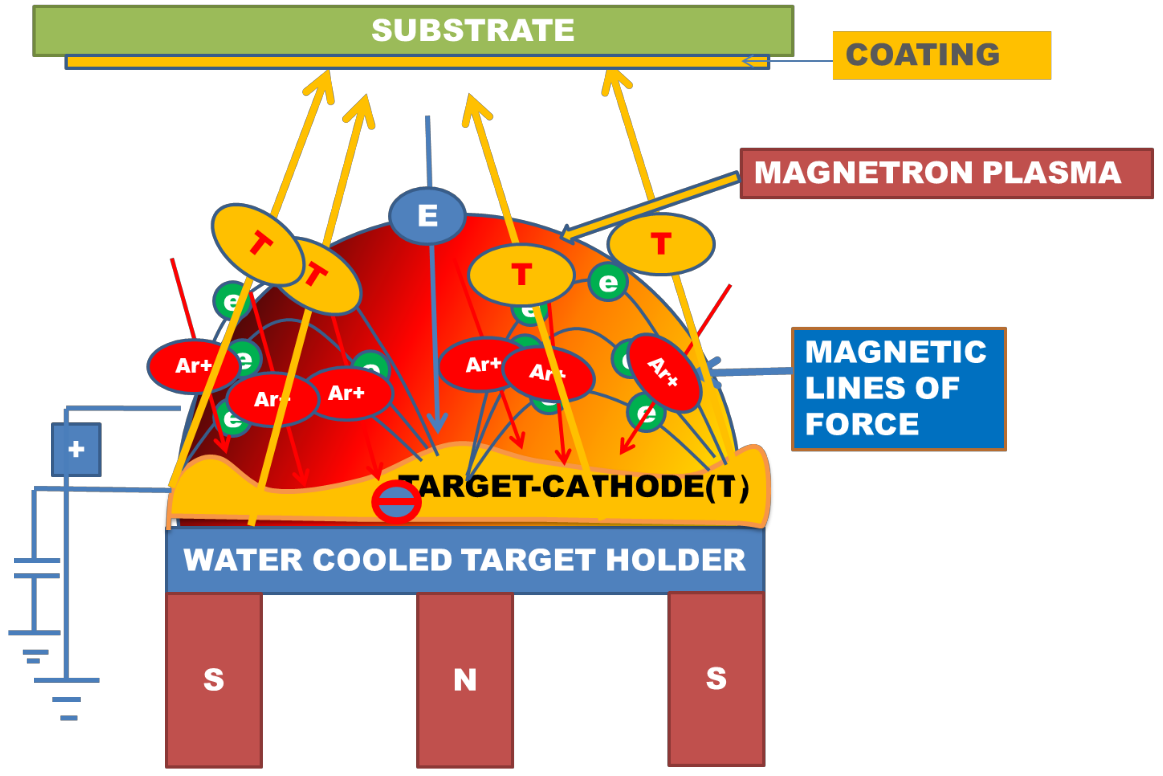
\includegraphics[width=12cm, height=8cm]{magnetron sputtering.png} \caption{Magnetron Sputtering system. credit: \cite{SurfaceEng}}
		\end{center}
	\end{figure}
	
	\subsection{Magnetic Mirror}
	The magnetic mirror effect can first be illustrated with a 	single particle. For the simple case, it is assumed that there is no electric field acting on the particle, the magnetic field is cylindrically symmetric and the gradient of the magnetic field is only along the axial direction of the cylinder, the $z$ direction.  The magnetic moment $$\mu = \frac{m v_{\perp}^{2}}{2B_{z}} $$ of the particle is an adiabatic invariant of the particle motion and hence is approximately conserved for a magnetic field whose $z$ component $B_{z}$ does not vary too much . The kinetic energy$$ KE = \frac{1}{2}m v^{2}$$ of the particle is also approximately conserved. Writing $v_{\perp} = v sin \theta$,
	$$\frac{\mu}{KE} = \frac{sin^{2}\theta}{B_{z}}$$ is also a conserved quantity. This means that as $B$ increases (within a small range), $sin^{2}\theta$ increases as well and so does $|sin\theta|$ which means that $|v_{\perp}|$ increases and since $v$ is conserved, $v_{\parallel}$ decreases to zero. When $v_{\parallel} = 0$, the particle is no longer moving in the $z$ direction, but is moving with velocity $v$ in the plane perpendicular to $z$ direction. The $v_{\parallel}$ then increases in the opposite direction as the particle moves towards decreasing $B$ because of the Lorentz force. Such a particle is seen as being reflected due to the configuration of the magnetic field and hence such a configuration of the magnetic field is called a magnetic mirror. Particles whose $v_{\parallel}$ does not decrease to 0 while the value of $B$ is decreasing, escape from the magnetic mirror configuration. \\
	
	\noindent A magnetic mirror configuration is important in a magnetic plasma trap chamber such as that used in Magnetron sputtering. Particles in a plasma have different speeds depending on the initial distribution which is based on parameters like the plasma temperature. The speeds of particles change depending on the electric and magnetic fields. Based on the magnetic mirror effect, one can determine which particle (having certain velocities) can escape the magnetic trap and which of those are reflected. The less the particles escape the magnetic trap, the more of the flux is used in forming coatings and less of the ionized gas is wasted. This is very useful in understanding the required gas supply and rate of deposition.
	
	\section{Literature Review}
	
	\subsection{Plasma as a system}
	Various models are used to describe Plasma as a system. Some of the common approaches are:
	\begin{enumerate}
		\item \textbf{Single particle description} \\
		This model is used to describe the motion of a charged particle under the influence of electric and magnetic fields. The particle's motion is described by the Lorentz force 
		\begin{equation}
			\label{eqn:lorentz}
			\frac{d \textbf{$\boldsymbol{v}$}}{d t} = \frac{q}{m} \left(\textbf{$\mathbf{E}$} + \textbf{$\boldsymbol{v}$} \times \textbf{$\mathbf{B}$} \right)
		\end{equation}
		Describing many particles evolving under the influence of Lorentz force, it is easy to describe a plasma assuming that the mean free path of the particles is much larger than the dimensions of the chamber; meaning that particles hardly ever collide.
	
		\item \textbf{Kinetic theory} \\
		The kinetic theory describes the plasma as collection of particles whose state (position and velocity) is treated as a random variable with a density function \\ $ f(x, y, z, v_{x}, v_{y}, v_{z}, t) $ which describes the number of particles at position $ (x, y, z) $ at time $ t $ with velocities between $ v_{x} $ and $ v_{x} + dv_{x} $, $ v_{y} $ and $ v_{y} + dv_{y} $, $ v_{z} $ and $ v_{z} + dv_{z} $ in directions $x$, $y$ and $z$ respectively. For a simpler notation $ f(x, y, z, v_{x}, v_{y}, v_{z}, t) $ is denoted as $ f(\boldsymbol{r}, \boldsymbol{v}, t) $.
		The expression $$\displaystyle \int_{all \hspace{0.2cm} v_{x}^{}} dv_{x} \int_{all \hspace{0.2cm} v_{y}^{}} dv_{y} \int_{all \hspace{0.2cm} v_{z}^{}} dv_{z} f(\boldsymbol{r}, \boldsymbol{v}, t) $$ gives the number of particles at position $\boldsymbol{r}$, at time $t$.  For a simple choice of notation, it if often written as $$\displaystyle \int_{all \hspace{0.2cm} \boldsymbol{v}^{}} d^{3}v f(\boldsymbol{r}, \boldsymbol{v}, t) \hspace{0.5cm}\mathnormal{or} \hspace{0.5cm}\int_{all \hspace{0.2cm} \boldsymbol{v}^{}} d\boldsymbol{v} f(\boldsymbol{r}, \boldsymbol{v}, t)$$ A density function is said to be normalized if $$\displaystyle \int_{all \hspace{0.2cm} \boldsymbol{v}^{}} d\boldsymbol{v} f(\boldsymbol{r}, \boldsymbol{v}, t) = 1$$ Such a density function is also denoted with a hat as $ \hat{f}(\boldsymbol{r}, \boldsymbol{v}, t) $.\\
		\noindent The average velocity $\bar{v}$ for a density function $ \hat{f}(\boldsymbol{r}, \boldsymbol{v}, t) $ is calculated as  $$\displaystyle \int_{all \hspace{0.2cm} \boldsymbol{v}^{}} d\boldsymbol{v} \hspace{0.2cm} v f(\boldsymbol{r}, \boldsymbol{v}, t)$$ Various other features of the distribution are: the Root Mean Square velocity $v_{rms}$, the average absolute velocity $|\bar{v}|$, the average velocity in $z$ direction $\bar{v_{z}}$, etc.\\
		The evolution of the particles is described as the changing of the density function. Boltzmann equation is often used to describe this dynamics:
		
		$$\frac{\partial f}{\partial t} + \boldsymbol{v} \cdot \nabla f + \frac{\mathbf{F}}{m} \cdot {\partial}_{\boldsymbol{v}} f = \left(\frac{\partial f}{\partial t}\right)_{c}$$
		\item \textbf{Fluid model} \\
		
		\item \textbf{Magnetohydrodynamics} \\
	\end{enumerate}
	
	\section{Gaps in Literature}
	
	\subsection{Particle in Cell Methods}
	
	\subsection{Boris Algorithm}
	
	\section{Problem Definition}
	
	\subsection{Particle Sampling}
	Maxwell Boltzmann distribution
	
	Parabolic density functions
	
	\subsection{Particle Evolution}
	Lorentz force and Boris Algorithm.
	
	\subsection{Fields}
	
	\section{Objectives}
	
	\section{Methodology}
	
	\section{Work carried out so far}
	
	\subsection{Algorithm Outline}
	
	\section{Work to be done}
	
	\section{Gantt Chart(Work Plan)}
	
	\section{Milestones in the project phase}
	
	\begin{thebibliography}{}
		\bibitem{SurfaceEng}
		Professor Sitaram Dash. (Fall Semester 2021). \textit{MEE4005 Surface Engineering} (lecture notes). SMEC, VIT Vellore.
		\bibitem{MKunz}
		Matthew W. Kunz. (November 9, 2020). \textit{Introduction to Plasma Astrophysics} (lecture notes). Princeton Plasma Physics Laboratory.
		\bibitem{chenbook}
		Chen, F. F. (1984). \textit{Introduction to plasma physics and controlled fusion} (Vol. 1, pp. 8-11). New York: Plenum press.
		\bibitem{mirror1}
		Na, Yong-Su (2017). \textit{Introduction to nuclear fusion} (Lecture 9 Mirror, lecture slide). Seoul National University Open Courseware.
		\bibitem{mirror2}
		F\"{o}rel\"{a}sning (2009). \textit{Charged particle motion in magnetic field} (lecture slide). Lule\"{a} University of Technology.
		\bibitem{Borisgood}
		Qin, H., Zhang, S., Xiao, J., $\&$ Tang, W. M. (April, 2013). \textit{Why is Boris algorithm so good?}. Princeton Plasma Physics Laboratory, PPPL-4872.
		
	\end{thebibliography}

\end{document}